\section{Conclusions}

We propose two measures of revision quality computed
from Wikipedia's revision history.
The measure \textit{text longevity} is based on an intuitive
model of computing the text added by authors at each revision
and detecting how much of that text remains within the article
in subsequent revisions; to account for the variation in
the amount of preserved text over the subsequent revisions,
we model the change as a geometrically decaying process
and compute the decay rate as a single value to describe
the variation.
The measure \textit{edit longevity} was developed to address
the reality that authors also delete and rearrange text,
and that these are valuable contributions to the Wikipedia.
Using edit distance~\cite{Levenshtein1966} to describe the
amount of \intro{effort} that an author puts into making a
revision to an article; we use this as the basis for computing
edit longevity by estimating the amount of effort by an
author that brings the article text closer to some future
version of the article.

We evaluate these two measures using the PAN-WVC-10 dataset, which is
manually annotated to indicate which revisions are vandalism and which
are well-intentioned edits, and treat each as a predictor of vandalism.
We find that edit longevity performs much better than text longevity,
but even text longevity does better than chance at predicting vandalism.
Overall, these results are encouraging for using edit longevity and text
longevity as signals for inferring the community feedback of an author's
edit.  Knowing the quality of edits, we can build an author reputation
system upon these signals; we describe such a system in
Chapter~\ref{ch:reputation}.

\subsection{Edit Longevity Outperforms Text Longevity}

In comparison to edit longevity, the performance of ${\approx}29.26\%$
PR-AUC is quite poor.
Why does text longevity not do so well as edit longevity?
As part of our investigation, we started looking at specific
instances of text longevity values.
In Figures~\ref{fig:ts-GeorgeWBush} and~\ref{fig:ts-SantaCruzBeachBoardwalk},
we see the text survival for two different contributions;
both do seem to have the general ``exponential'' shape
that we previously described.
Also computed in each figure is the text longevity measure based on
the 20~revisions shown in each graph, but notice that the text
longevity computed for
Figure~\ref{fig:ts-GeorgeWBush} doesn't exhibit the curve we expect.

\begin{figure}[tbph]
\centering
\framebox{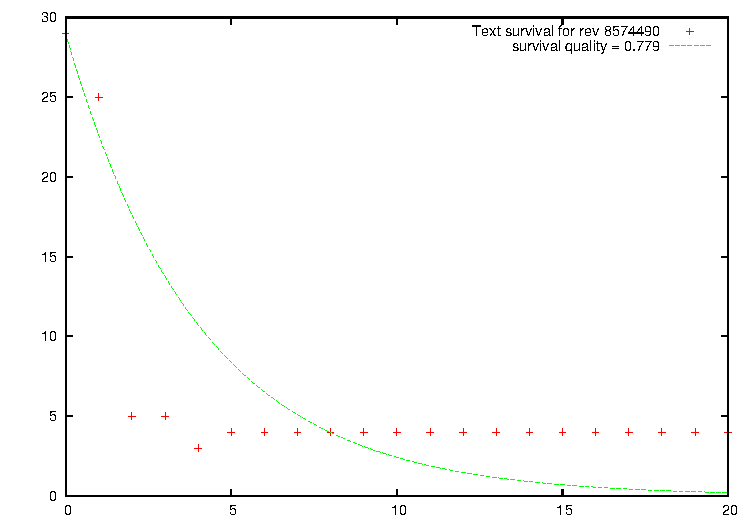
\includegraphics[width=0.8\textwidth]{part-F70-editquality/graph-TS-GeorgeWBush-8574490}}
\caption{The text survival graph for the text contributed early
        in the history of article \textit{George W.~Bush}.
	The graph also shows the text survival quality
	computed based on 20~revisions.
	}
\label{fig:ts-GeorgeWBush}
\end{figure}

\begin{figure}[tbph]
\centering
\framebox{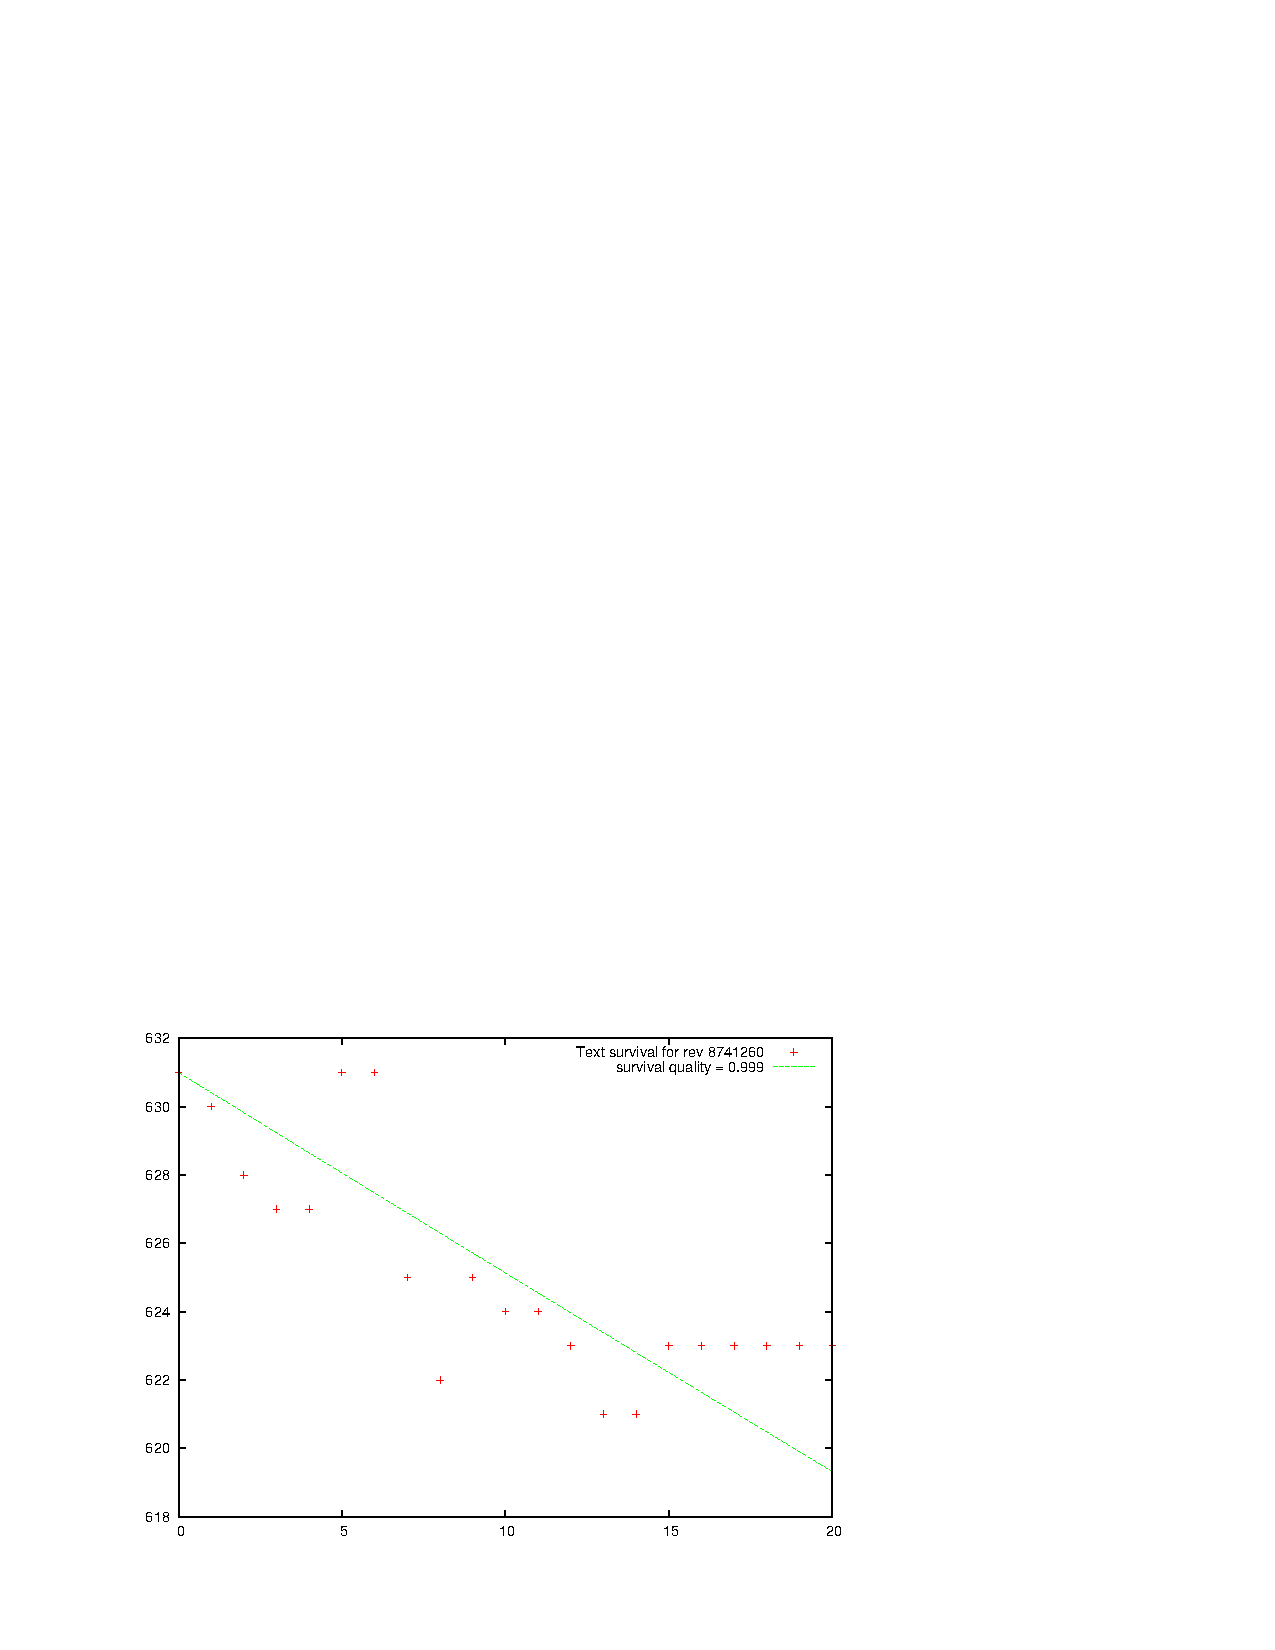
\includegraphics[width=0.8\textwidth]{part-F70-editquality/graph-TS-SantaCruzBeachBoardwalk}}
\caption{The text survival graph for the text initially contributed
	as part of the article \textit{Santa Cruz Beach Boardwalk}.
	The majority of the editing to the contributed text happens
	in the next few revisions, before the text stabilizes.
	The graph also shows the text survival quality
	computed based on 20~revisions.
	}
\label{fig:ts-SantaCruzBeachBoardwalk}
\end{figure}

The explanation for this discrepancy turns out to be a flaw in our
thinking about the original model.
While the text survival for contributions does seem to have an
exponential look to it, exponentials do not approach some fixed
non-zero value --- they approach zero.
In order to fit the curve we are describing, the last value
(in the case of the data shown in Figure~\ref{fig:ts-GeorgeWBush},
the amount of text that survives after the $20^{th}$ revision)
should be taken as the ``zero reference point'' which is subtracted
from all the values.
Applying our exponential curve fitting technique to these new values
will give a much better approximation to the data.
The problem with this better fit is that it changes the meaning of
a score of zero; instead of meaning that the text was immediately deleted,
a score of zero would mean that the text immediately reached its
final survival level.
In other words, we would be measuring how quickly the text stabilizes,
rather than how much agreement there was that the text belonged in
the article.

\subsection{Triangle Inequality}


Whatever weight we choose for insertions and deletions in the edit
distance computation, we know that the author took some
\textit{explicit} action to effect the insertion or deletion.
The same is not true for the Move operation: our use of
Tichy's block moves~\cite{Tichy1984} obscures the information
about what text stays in the same relative order in the
transformation from the old revision to the new revision.

\mynote{TODO: Continue this line of thinking and reference
Sankoff and discuss reverse triangle inequality.}

